\documentclass[utf8x]{G7-32} % Стиль (по умолчанию будет 14pt)

\usepackage{amsmath,amssymb,amsfonts}
\usepackage{algorithmic}
\usepackage{graphicx}
\usepackage{textcomp}
\usepackage{multirow}
\usepackage{xcolor}
\usepackage{subcaption}
\usepackage{lipsum}
\usepackage{float}
\renewcommand\thesubfigure{\asbuk{subfigure}}

\usepackage{tikz}
\usepackage{pgfplots}
\usetikzlibrary{spy,calc}
\newlength\imagewidth
\newlength\imagescale

\pagestyle{empty}

\begin{document}
	
	\begin{figure}[H]
		\centering
		\begin{subfigure}{\textwidth}
			\centering
			\caption{}
			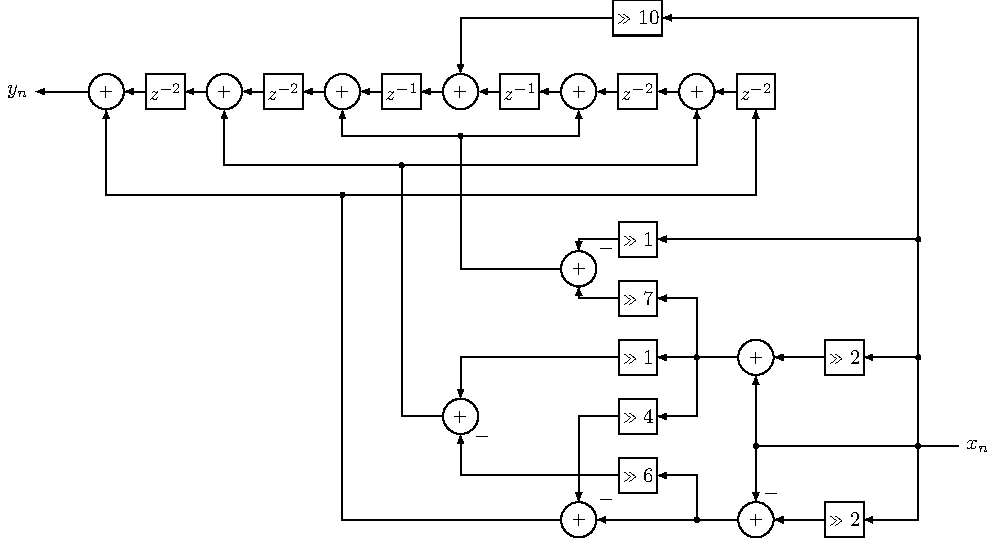
\includegraphics[width=1\linewidth]{hbf_12_reduced_transposed_mcm.pdf}
			\label{fig:Res4_hbf94_scheme1}
		\end{subfigure}%
		\vspace{1cm}  % Расстояние между изображениями, можно настроить
		\begin{subfigure}{\textwidth}
			\centering
			\caption{}
			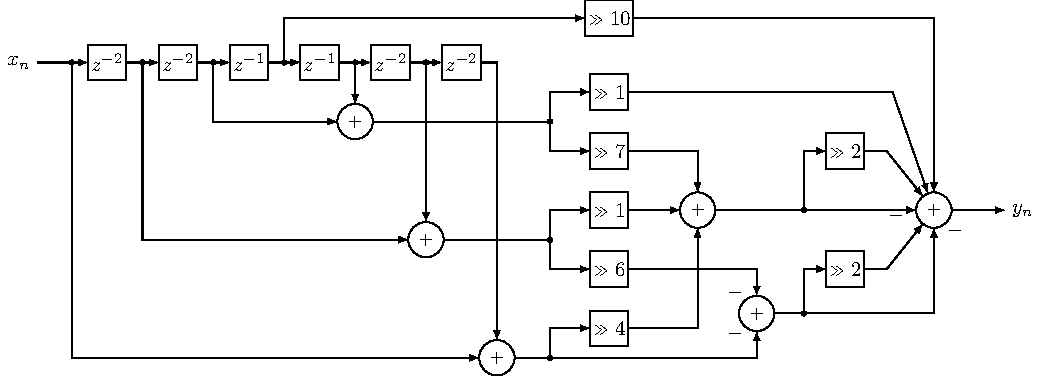
\includegraphics[width=1\linewidth]{hbf_12_reduced_mcm.pdf}
			\label{fig:Res4_fmr_scheme1}
		\end{subfigure}
		%	\caption{(а) --- АЧХ изначального и упрощенного ППФ 30 порядка и ошибка между ними; (б) --- АЧХ изначального и упрощенного ФНЧ 94 порядка и ошибка между ними}
	\end{figure}
	
	
\end{document}